\section{Experimental Study}
\label{sec-exp}

We evaluate \hermes on three questions.
\textbf{[RQ1] Effectiveness}: how accurate is operator-level planning
against one-shot generation and constraint-guided search, at the same
model and on the same graph store?
\textbf{[RQ2] Components}: what do the verifier, the execution feedback,
and the reference answers contribute?
\textbf{[RQ3] Cost}: how many model calls, graph executions, and how
much time does each method spend?
All configurations, run outputs, and the scripts that build every table
and figure here from them are in the artifact.

\subsection{Experimental Setup}

\stitle{Benchmarks}.
We normalize six benchmarks into one format
(Table~\ref{tab-bench}): every question and language becomes one item
with its gold query, feature tags (\eg \kw{COUNT}, \kw{GROUP},
\kw{ORDER}, \kw{ASK}), and gold answers stored as in the official
Text2SPARQL scorer.
Sources are pinned to commits and checksums.
This paper reports CK26, the corporate track of the Text2SPARQL 2026
challenge~\cite{text2sparql}; DB26, its DBpedia track, is in progress.
CK26 asks 50 questions in English and German over a corporate graph of
products, suppliers, and employees (13 classes, 30 properties, about
26.6k triples), loaded locally; DB26 asks 50 questions in English and
Spanish over DBpedia~\cite{auer2007dbpedia}, queried at the organizers'
endpoint.
Each track has 100 items.

\begin{table}[t]
  \caption{Normalized benchmarks. Items are question--language pairs.}
  \label{tab-bench}
  \small
  \begin{tabular}{@{}lrrl@{}}
    \toprule
    Benchmark & Questions & Items & Graph \\
    \midrule
    CK26~\cite{text2sparql} & 50 & 100 & corporate, local \\
    DB26~\cite{text2sparql} & 50 & 100 & DBpedia, endpoint \\
    CK25~\cite{text2sparql2025} & 50 & 50 & corporate, local \\
    DB25~\cite{text2sparql2025} & 100 & 200 & DBpedia, endpoint \\
    QALD-10~\cite{qald10} & 394 & 1,564 & Wikidata, live \\
    QALD-9-plus~\cite{qald9plus} & 150 & 450 & DBpedia, live \\
    \bottomrule
  \end{tabular}
\end{table}

\stitle{Data caveats}.
Three properties of the data shape what a number means.
(1) Forty-nine of the fifty CK26 gold queries appear verbatim in CK25, on
the same graph, so neither is a development set for the other; no
method here uses either for examples or tuning.
(2) The CK gold answers were computed on the Tentris engine.
Rerunning the gold queries on Oxigraph reproduces 43 of the 50; the
other seven differ in tie-breaking under \kw{LIMIT}, decimal formatting,
or the non-standard cast \kw{xsd{:}int()}.
We report results on all items and on the 86 items whose gold
reproduces.
All 50 DB26 gold queries reproduce on the organizers' endpoint.
(3) The official scorer has two quirks for ASK and ordered questions,
described in Appendix~C; we report the official metric and a strict
variant that corrects them.

\stitle{Metrics}.
We report set precision (P), recall (R), and $F_1$, and the challenge's
ranking metric $F_{\mathrm{ndcg}}$, which uses nDCG on questions whose
order matters and set $F_1$ elsewhere.
Our scorer reproduces all 5,024 per-question and average scores
published for the 2026 challenge (Appendix~C), so our numbers are on
the leaderboard's scale.

\stitle{Methods}.
\emph{OneShot} prompts a single query from the schema vocabulary,
declares any known prefix the draft omits, and makes one repair call if
the draft does not parse.
\emph{CGS} is our reimplementation of constraint-guided search with
Chase and Backchase~\cite{wang2026uniqgen}.
It follows the published three stages, with two documented deviations:
queries are rendered from constraints deterministically rather than by
a second model, and candidates are scored by comparing answer sets with
the reference answers rather than by a model.
It uses two model calls per question, one for the constraint table and
one for the reference answers, beam width 5, and depth 5.
\emph{\hermes{}$^-$} is the planner of Section~\ref{sec-framework} with
the verifier disabled: execution feedback, no typing, no goal.
\emph{\hermes} is the full verified planner.
Both planners have a step budget of $B = 15$, and their prompt examples
use an unrelated domain (Olympic host cities, Figure~\ref{fig-prompt});
no prompt names CK26 content.

\stitle{Models}.
We run every method with Qwen3~\cite{yang2025qwen3} at three sizes,
4B, 8B, and 14B parameters, with thinking disabled and temperature 0.
Each model is served in bf16 by vLLM~\cite{kwon2023vllm} on one NVIDIA
L40S GPU, and each run sends 16 items at a time so that the server
batches their requests.
Replies are capped at 2,048 tokens.
Small open models keep every run reproducible at low cost and keep
differences between methods from being masked by a model that answers
from memory; the published Text2SPARQL entries use larger models, so
our numbers are a lower bound for each method.
\hermes takes the model as a parameter, so the same runs extend to other
open models such as Llama~3.1~\cite{grattafiori2024llama3} and to API
models such as GPT-4~\cite{openai2023gpt4}.
\warn{[Pending: API models and Llama~3.1 8B.]}

\stitle{Implementation}.
All methods share the graph store (Oxigraph, in memory), the entity
index, and the scorer.
Every graph query is limited to 30\,s and every item to 300\,s; an item
that exceeds its limit counts as unanswered.
Runs record the source commit, and each table and figure in this
section is generated from the committed run outputs.

\subsection{RQ1: Effectiveness}

Table~\ref{tab-main} reports all twelve runs.
\hermes is the most accurate method at 14B: $F_1$ 0.282, against 0.231
for \hermes{}$^-$, 0.197 for CGS, and 0.089 for OneShot, with the highest
precision (0.290), recall (0.414), and $F_{\mathrm{ndcg}}$.
It answers 16 items exactly, as many as \hermes{}$^-$, against 11 for
CGS and 4 for OneShot.
The lead holds in both languages ($F_1$ 0.297 in English and 0.268 in
German, against 0.274 and 0.187 for \hermes{}$^-$) and on the 86 items
whose gold reproduces (0.297).
Strict scoring changes no $F_1$ at any size, because no method answers
an ASK question.

\begin{table}[t]
  \caption{Effectiveness on CK26 (100 items). Official metrics; Strict
    is set $F_1$ under the corrected scorer, and Repro.\ is set $F_1$ on
    the 86 items whose gold reproduces. Best per model in bold.}
  \label{tab-main}
  \footnotesize
  \setlength{\tabcolsep}{3.2pt}
  % Generated by experiments/tables.py from results/; do not edit.
\begin{tabular}{@{}llrrrrrr@{}}
\toprule
Model & Method & P & R & $F_1$ & $F_{\mathrm{ndcg}}$ & Strict & Repro. \\
\midrule
\multirow{4}{*}{Qwen3-4B} & OneShot & 0.001 & 0.000 & 0.000 & 0.000 & 0.000 & 0.000 \\
 & CGS & 0.094 & 0.169 & 0.084 & 0.085 & 0.084 & 0.082 \\
 & \cellcolor{hermesbg}\hermes{}$^-$ & \cellcolor{hermesbg}\textbf{0.099} & \cellcolor{hermesbg}0.167 & \cellcolor{hermesbg}\textbf{0.103} & \cellcolor{hermesbg}\textbf{0.102} & \cellcolor{hermesbg}\textbf{0.103} & \cellcolor{hermesbg}\textbf{0.114} \\
 & \cellcolor{hermesbg}\hermes & \cellcolor{hermesbg}0.064 & \cellcolor{hermesbg}\textbf{0.207} & \cellcolor{hermesbg}0.070 & \cellcolor{hermesbg}0.071 & \cellcolor{hermesbg}0.070 & \cellcolor{hermesbg}0.080 \\
\midrule
\multirow{4}{*}{Qwen3-8B} & OneShot & 0.093 & 0.068 & 0.067 & 0.068 & 0.067 & 0.078 \\
 & CGS & 0.155 & 0.262 & 0.121 & 0.121 & 0.121 & 0.119 \\
 & \cellcolor{hermesbg}\hermes{}$^-$ & \cellcolor{hermesbg}\textbf{0.168} & \cellcolor{hermesbg}0.372 & \cellcolor{hermesbg}\textbf{0.178} & \cellcolor{hermesbg}\textbf{0.178} & \cellcolor{hermesbg}\textbf{0.178} & \cellcolor{hermesbg}\textbf{0.182} \\
 & \cellcolor{hermesbg}\hermes & \cellcolor{hermesbg}0.148 & \cellcolor{hermesbg}\textbf{0.412} & \cellcolor{hermesbg}0.158 & \cellcolor{hermesbg}0.159 & \cellcolor{hermesbg}0.158 & \cellcolor{hermesbg}0.172 \\
\midrule
\multirow{4}{*}{Qwen3-14B} & OneShot & 0.111 & 0.091 & 0.089 & 0.090 & 0.089 & 0.103 \\
 & CGS & 0.209 & 0.399 & 0.197 & 0.197 & 0.197 & 0.210 \\
 & \cellcolor{hermesbg}\hermes{}$^-$ & \cellcolor{hermesbg}0.254 & \cellcolor{hermesbg}0.277 & \cellcolor{hermesbg}0.231 & \cellcolor{hermesbg}0.231 & \cellcolor{hermesbg}0.231 & \cellcolor{hermesbg}0.251 \\
 & \cellcolor{hermesbg}\hermes & \cellcolor{hermesbg}\textbf{0.290} & \cellcolor{hermesbg}\textbf{0.414} & \cellcolor{hermesbg}\textbf{0.282} & \cellcolor{hermesbg}\textbf{0.282} & \cellcolor{hermesbg}\textbf{0.282} & \cellcolor{hermesbg}\textbf{0.297} \\
\bottomrule
\end{tabular}

\end{table}

Accuracy grows with model size for every method (Figure~\ref{fig-sizes}),
but not at the same rate.
From 4B to 14B, $F_1$ rises by 0.212 for \hermes, 0.128 for
\hermes{}$^-$, 0.113 for CGS, and 0.089 for OneShot.
At 4B, CGS is the most accurate method (0.084 $F_1$ against 0.070 for
\hermes): the planners need a model that can follow a multi-step
protocol, and the 4B model often does not (Section~\ref{sec-exp-rq2}).
OneShot at 4B scores 0: on 79 items its query does not parse, most
often because it omits the query form (\kw{SELECT}).

\begin{figure}[t]
  \centering
  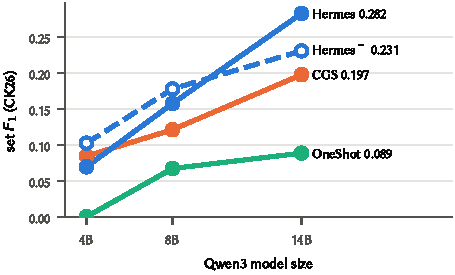
\includegraphics[width=\columnwidth]{fig/sizes.pdf}
  \caption{Set $F_1$ on CK26 against Qwen3 model size. Dashed, hollow:
    \hermes without the verifier.}
  \label{fig-sizes}
\end{figure}

For scale, Table~\ref{tab-peers} places the 14B runs among the
published 2026 entries on CK26, which range from 0.157 to 0.832 in
$F_{\mathrm{ndcg}}$~\cite{smeros2026sparqlllm,text2sparql}.
This is not a paired comparison: those systems were scored by the
organizers on Tentris, and their models are not controlled here.
With a 14B open model, \hermes places above three of the eight
entries.

\begin{table}[t]
  \caption{CK26 $F_{\mathrm{ndcg}}$ of the published Text2SPARQL 2026
    entries, scored by the organizers, and of our runs with Qwen3-14B
    (shaded).}
  \label{tab-peers}
  \small
  \begin{tabular}{@{}lr@{\hspace{2em}}lr@{}}
    \toprule
    Entry & $F_{\mathrm{ndcg}}$ & Entry & $F_{\mathrm{ndcg}}$ \\
    \midrule
    SPARQL-LLM~\cite{smeros2026sparqlllm} & \textbf{0.832} & \cellcolor{hermesbg}\hermes{}$^-$ & \cellcolor{hermesbg}0.231 \\
    INFAI-ETI-A & 0.633 & IRIS & 0.217 \\
    ADFR & 0.513 & LIBER-AI-QWEN & 0.206 \\
    INFAI-ETI-C & 0.452 & \cellcolor{ours}CGS & \cellcolor{ours}0.197 \\
    LIBER-AI-CLAUDE & 0.335 & INFAI-ETI-B & 0.157 \\
    \cellcolor{hermesbg}\hermes & \cellcolor{hermesbg}0.282 & \cellcolor{ours}OneShot & \cellcolor{ours}0.090 \\
    \bottomrule
  \end{tabular}
\end{table}

Table~\ref{tab-features} breaks the 14B runs down by the feature tags
of the gold queries.
\hermes leads on plain selections, filters, and nested queries.
\hermes{}$^-$ leads on ordering, grouping, counting, and slicing.
No method answers any of the six ASK items.

\begin{table}[t]
  \caption{CK26 set $F_1$ by feature tag of the gold query (Qwen3-14B);
    a question can carry several tags, and $n$ counts items. Best per
    row in bold.}
  \label{tab-features}
  \small
  % Generated by experiments/tables.py from results/; do not edit.
\begin{tabular}{@{}lrrrrr@{}}
\toprule
Tag & $n$ & OneShot & CGS & \hermes{}$^-$ & \hermes \\
\midrule
\kw{SELECT} & 94 & 0.094 & 0.210 & \cellcolor{hermesbg}0.245 & \cellcolor{hermesbg}\textbf{0.300} \\
\kw{FILTER} & 10 & 0.096 & 0.391 & \cellcolor{hermesbg}0.285 & \cellcolor{hermesbg}\textbf{0.395} \\
\kw{ORDER} & 30 & 0.030 & 0.092 & \cellcolor{hermesbg}\textbf{0.174} & \cellcolor{hermesbg}0.131 \\
\kw{SUBSELECT} & 8 & 0.047 & \zero & \cellcolor{hermesbg}0.001 & \cellcolor{hermesbg}\textbf{0.094} \\
\kw{GROUP} & 18 & \zero & 0.081 & \cellcolor{hermesbg}\textbf{0.168} & \cellcolor{hermesbg}0.156 \\
\kw{COUNT} & 16 & \zero & 0.089 & \cellcolor{hermesbg}\textbf{0.244} & \cellcolor{hermesbg}0.165 \\
\kw{LIMIT} & 26 & \zero & 0.063 & \cellcolor{hermesbg}\textbf{0.115} & \cellcolor{hermesbg}0.065 \\
\kw{ASK} & 6 & \zero & \zero & \cellcolor{hermesbg}\zero & \cellcolor{hermesbg}\zero \\
\bottomrule
\end{tabular}

\end{table}

\subsection{RQ2: Components}
\label{sec-exp-rq2}

\stitle{Verifier}.
Table~\ref{tab-verifier} compares \hermes with \hermes{}$^-$, which
differ only in the verifier.
The verifier sharply reduces the items that end with no runnable query
at every size: from 57 to 35 at 4B, from 15 to 2 at 8B, and from 26 to
9 at 14B.
It rejects 37, 48, and 29 steps per run at 4B, 8B, and 14B, and each
rejection names the violated rule (for example, a projected variable
that no pattern binds), so the planner repairs the step instead of
running it.
Accuracy follows at 14B, where $F_1$ rises from 0.231 to 0.282.
At 4B and 8B it does not: $F_1$ falls from 0.103 to 0.070 and from
0.178 to 0.158.
At 4B, \hermes returns a query on 30 items where \hermes{}$^-$ returned
none, but only 10 of them score above zero, and it scores zero on 11
items that \hermes{}$^-$ answered in part; at 8B the counts are 14, 6,
and 16.
The verifier turns failures into answers; whether the answers are
right depends on the model.

\begin{table}[t]
  \caption{The verifier: \hermes against \hermes{}$^-$ on CK26. No
    answer counts items that end without a runnable query; Steps is the
    mean number of actions per item.}
  \label{tab-verifier}
  \footnotesize
  \setlength{\tabcolsep}{3.5pt}
  % Generated by experiments/tables.py from results/; do not edit.
\begin{tabular}{@{}lrrrrrr@{}}
\toprule
& \multicolumn{2}{c}{$F_1$} & \multicolumn{2}{c}{No answer} & \multicolumn{2}{c}{Steps} \\
\cmidrule(lr){2-3}\cmidrule(lr){4-5}\cmidrule(l){6-7}
Model & \hermes{}$^-$ & \hermes & \hermes{}$^-$ & \hermes & \hermes{}$^-$ & \hermes \\
\midrule
Qwen3-4B & \textbf{0.103} & 0.070 & 57 & \textbf{35} & 5.6 & 9.3 \\
Qwen3-8B & \textbf{0.178} & 0.158 & 15 & \textbf{2} & 11.2 & 13.7 \\
Qwen3-14B & 0.231 & \textbf{0.282} & 26 & \textbf{9} & 10.3 & 11.3 \\
\bottomrule
\end{tabular}

\end{table}

\stitle{Reference answers}.
CGS ranks candidates by their agreement with reference answers that the
model predicts.
\warn{[Pending: CGS with gold reference answers on Qwen3.]}

\stitle{Feedback signals}.
\warn{[Pending: ablation of the observation, removing in turn the
count, the change in count, the row sample, and the error message.]}

\subsection{RQ3: Time and Cost}
\label{sec-exp-rq3}

Table~\ref{tab-cost} reports the cost of every run; Figure~\ref{fig-cost}(a)
sets accuracy against model calls, and Figure~\ref{fig-cost}(b) shows
the time of every item.
All twelve runs take 27.6 minutes of L40S time in total.

\stitle{Model calls and tokens}.
The planners spend 12.7 to 14.6 model calls per item, against about 2
for CGS and 1 to 2 for OneShot, and read about 28k input tokens per
item, 7 times as many as CGS: every step resends the plan and its
observations.
Output is small for all methods (11k to 52k tokens per run), so input
dominates the cost.
The comparison in Table~\ref{tab-main} is therefore not at equal model
budget.
\warn{[Pending: budget-matched comparison, \eg CGS or OneShot with
self-consistency at 15 calls per item.]}

\stitle{Budgeted planning}.
Table~\ref{tab-budget} runs the budgeted planner of
Section~\ref{sec-framework} with Llama~3.1 8B~\cite{grattafiori2024llama3},
served locally through Ollama~\cite{ollama}, against the other methods
under the same model, with a budget of three model calls and eight
candidate executions per item.
Its binding repairs were designed while reading the traces of CK26
questions 1 to 10, so the table also reports questions 11 to 50 (80 items)
as a held-out split.
On that split the planner scores 0.089, against 0.081 for \hermes{}$^-$,
with 2.15 model calls per item instead of 14.51, in half the wall time;
the difference is small for 80 items.
Selection is not the bottleneck: the chosen candidates score 0.111, and
the best candidate the planner ever generated would score 0.113.
The confidence $p(Q)$ ranks candidates well: the top tenth of executed
candidates by $p$ have a mean $F_1$ of 0.425, against 0.047 for all of
them, and the 27 items the planner does not abstain on score 0.411.
What is missing is coverage: on 40 items no reading bound to a
well-typed plan.
On DB26 the planner scores 0.007, below OneShot (0.017); binding resolves
common DBpedia terms, but the model's readings of these longer questions
rarely contain the right structure, and only 1 of 527 executed
candidates is correct, too few to fit the selector.

\begin{table}[t]
  \caption{Budgeted planning on CK26 with Llama~3.1 8B. Held-out is
    questions 11--50 (80 items); Calls is model calls per item; Time is
    the run's wall time in minutes.}
  \label{tab-budget}
  \footnotesize
  \setlength{\tabcolsep}{4pt}
  \begin{tabular}{lrrrr}
    \toprule
    Method & $F_1$ & Held-out $F_1$ & Calls & Time \\
    \midrule
    OneShot & 0.017 & 0.009 & 1.16 & 6.2 \\
    CGS & 0.064 & 0.062 & 1.98 & 35.6 \\
    \hermes{}$^-$ & 0.094 & 0.081 & 14.51 & 40.4 \\
    \rowcolor{hermesbg} Budgeted & \textbf{0.111} & \textbf{0.089} & 2.15 & 21.2 \\
    \bottomrule
  \end{tabular}
\end{table}

\stitle{Time}.
Because the server batches 16 items at a time, every run of 100 items
finishes in 1.0 to 3.6 minutes.
Per item, the planners are slower and more predictable: at 14B the
median item takes 25.5\,s for \hermes and 21.7\,s for \hermes{}$^-$,
against 9.9\,s for CGS and 3.1\,s for OneShot, and the 95th percentile
is 32.7\,s for \hermes against 110.5\,s for CGS.
The step budget bounds each planner item, while the time of CGS depends
on the size of its search: at 14B it runs 2,132 graph executions,
more than twice as many as \hermes (902).

\begin{figure*}[t]
  \centering
  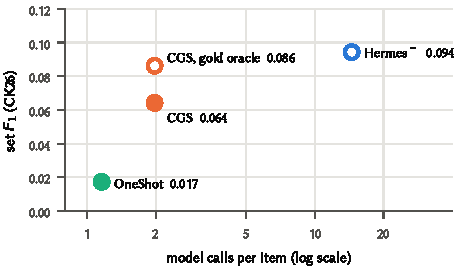
\includegraphics[width=\textwidth]{fig/cost.pdf}
  \caption{Cost on CK26 with Qwen3-14B. (a) Set $F_1$ against model
    calls per item. (b) Seconds per item, one dot per item, with the
    median as a bar. Hollow markers: \hermes without the verifier.}
  \label{fig-cost}
\end{figure*}

\begin{table}[t]
  \caption{Cost per run on CK26 (100 items). Calls are model calls;
    In and Out are input and output tokens in thousands; Exec.\ counts
    graph executions; Wall is the whole run in minutes; p50 and p95 are
    seconds per item.}
  \label{tab-cost}
  \footnotesize
  \setlength{\tabcolsep}{2.8pt}
  % Generated by experiments/tables.py from results/; do not edit.
\begin{tabular}{@{}llrrrrrrr@{}}
\toprule
Model & Method & Calls & In (k) & Out (k) & Exec. & Wall & p50 & p95 \\
\midrule
\multirow{4}{*}{4B} & OneShot & 198 & 91 & 16.8 & 21 & 1.1 & 2.7 & 3.6 \\
 & CGS & 180 & 419 & 39.9 & 995 & 1.6 & 3.2 & 54.0 \\
 & \cellcolor{hermesbg}\hermes{}$^-$ & \cellcolor{hermesbg}1,417 & \cellcolor{hermesbg}2,569 & \cellcolor{hermesbg}23.4 & \cellcolor{hermesbg}452 & \cellcolor{hermesbg}3.6 & \cellcolor{hermesbg}7.3 & \cellcolor{hermesbg}177.3 \\
 & \cellcolor{hermesbg}\hermes & \cellcolor{hermesbg}1,455 & \cellcolor{hermesbg}2,841 & \cellcolor{hermesbg}34.5 & \cellcolor{hermesbg}482 & \cellcolor{hermesbg}1.0 & \cellcolor{hermesbg}9.5 & \cellcolor{hermesbg}12.5 \\
\midrule
\multirow{4}{*}{8B} & OneShot & 111 & 76 & 12.8 & 87 & 1.8 & 2.3 & 4.8 \\
 & CGS & 196 & 430 & 51.3 & 635 & 2.8 & 7.0 & 80.9 \\
 & \cellcolor{hermesbg}\hermes{}$^-$ & \cellcolor{hermesbg}1,342 & \cellcolor{hermesbg}2,806 & \cellcolor{hermesbg}29.0 & \cellcolor{hermesbg}830 & \cellcolor{hermesbg}2.1 & \cellcolor{hermesbg}18.3 & \cellcolor{hermesbg}24.9 \\
 & \cellcolor{hermesbg}\hermes & \cellcolor{hermesbg}1,395 & \cellcolor{hermesbg}3,196 & \cellcolor{hermesbg}30.5 & \cellcolor{hermesbg}873 & \cellcolor{hermesbg}2.5 & \cellcolor{hermesbg}22.4 & \cellcolor{hermesbg}27.5 \\
\midrule
\multirow{4}{*}{14B} & OneShot & 106 & 73 & 11.3 & 93 & 3.0 & 3.1 & 9.3 \\
 & CGS & 199 & 392 & 27.3 & 2,132 & 2.7 & 9.9 & 110.5 \\
 & \cellcolor{hermesbg}\hermes{}$^-$ & \cellcolor{hermesbg}1,424 & \cellcolor{hermesbg}2,945 & \cellcolor{hermesbg}28.0 & \cellcolor{hermesbg}833 & \cellcolor{hermesbg}2.5 & \cellcolor{hermesbg}21.7 & \cellcolor{hermesbg}32.4 \\
 & \cellcolor{hermesbg}\hermes & \cellcolor{hermesbg}1,265 & \cellcolor{hermesbg}2,856 & \cellcolor{hermesbg}24.5 & \cellcolor{hermesbg}902 & \cellcolor{hermesbg}2.6 & \cellcolor{hermesbg}25.5 & \cellcolor{hermesbg}32.7 \\
\bottomrule
\end{tabular}

\end{table}

\subsection{Case Study}

Table~\ref{tab-case} is the trace of \hermes with Qwen3-14B on the
German version of Example~\ref{exa-motivation}.
The first action states the goal, one answer of type
\kw{pv{:}Department}, before any query exists.
The lookup returns two employees named Brant; the planner binds Karen
Brant, and the join with \kw{pv{:}memberOf} yields one solution of the
goal's type, the gold answer.
The verifier matters on other items.
On ``What's Baldwin Dirksen's phone number?'', \hermes{}$^-$ found the
employee but then tried to project the property \kw{pv{:}phone} as if it
were a variable, failed, and repeated the step until its budget ran
out; \hermes stated a literal goal, joined
\kw{pv{:}phone\ ?p}, and answered in four steps.
On a German request for every supplier's name and address, the verifier
rejected a projection of \kw{?addressText}, a variable whose pattern
the planner had removed because it matched nothing; the planner
projected the bound address fields instead and reached $F_1$ 0.84,
where \hermes{}$^-$ scored 0.

\begin{table}[t]
  \caption{Trace of \hermes (Qwen3-14B) on ``Zu welcher Abteilung
    gehört Frau Brant?'' (CK26, item 1, German).}
  \label{tab-case}
  \small
  \begin{tabular}{@{}lp{0.46\columnwidth}@{}}
    \toprule
    Action & Observation \\
    \midrule
    \kw{goal} \kw{?d} : \kw{pv{:}Department} & one answer \\
    \kw{lookup} ``Frau Brant'' & 2 entities: Karen, Sylvester Brant \\
    \kw{lookup} ``Karen Brant'' & 1 entity \\
    \kw{triple} \kw{?e\ pv{:}name}\ ``Karen Brant'' & 1 solution \\
    \kw{triple} \kw{?e\ pv{:}memberOf\ ?d} & 1 solution \\
    \kw{project} \kw{?d} & 1 solution \\
    \kw{finish} & accepted \\
    \bottomrule
  \end{tabular}
\end{table}
